\chapter{Trabalhos Relacionados}
	\label{ch:trabalhos}
Neste capítulo são discutidos alguns trabalhos que possuem um objetivo similar ao sistema produzido ou utilizam tecnologias similares. 

\section{Trabalhos menos relacionados}

O trabalho de \citeonline{gprsTelemetrySystem2013} propõe uma solução de telemetria para um veículo de competição elétrico. A proposta se assemelha ao trabalho proposto no quesito de manter a equipe em questão atualizada dos dados provindos do carro, a diferença é que o veículo é movido a energia limpa, elétrica. Este requisito altera também algumas das grandezas a serem analisadas pelo sistema, nele são verificados fatores como amperes por hora, voltagem, velocidade e distância percorrida. Infelizmente o trabalho não comenta como é feita a coleta dos dados pelos sensores, apenas comentando que existe um equipamento que faz o mesmo. Para parte de telemetria, os desenvolvedores comentam que trabalharam com foco em resolver dois problemas: robustez sobre todo o circuito de provas e segurança dos dados, além de redução do ruído. Portanto, duas tecnologias foram analisadas para a transmissão dos dados embarcados do veículo até os computadores da equipe, a de rádio frequência e a rede móvel de celular (GSM). A rede GSM foi escolhida sobre a rádio frequência devido a impossibilidade de garantir a comunicação entre todos os circuitos devido aos formatos e obstáculos encontrados no terreno, também é comentado que foram realizados testes e todos os circuitos possuem cobertura de sinal móvel. Por último, é desenvolvido um \textit{software} para receber os dados provenientes do veículo. O sistema de aquisição de dados teve seu funcionamento dividido em quatro blocos, sendo eles: configuração do aplicativo e do canal transmissão de dados usado; informações específicas da direção do piloto e do circuito percorrido; valores numéricos dos dados técnicos mais importantes para a manutenção do veículo em tempo real; representação gráfica de toda a informação recebida durante todo o processo da prova. Com isto e o tratamento das informações, o programa apresenta para a equipe de boxes informações como:

\begin{itemize}
	\item Consumo de energia; 
	\item Voltagem da bateria;
	\item Velocidade;
	\item Distância percorrida; e
	\item Eficiência energética.
\end{itemize}

Todas estas informações disponíveis são relevantes, porém o artigo não entra em detalhes quanto a construção do sistema de aquisição, o que pode aumentar em muito a relevância deste trabalho para o projeto proposto. Como é comentado, existe um indício de emprego de técnicas de engenharia de \textit{software} na criação do sistema de aquisição de dados, porém por não ser o foco do trabalho, as mesmas não são citadas. 

Outro trabalho que também possui um carro movido a energia limpa e propõe um sistema de aquisição de dados é o de \citeonline{applicationOfData2010}. O sistema é desenvolvido para um carro que utilizada um motor elétrico e deve ser capaz de percorrer distâncias de mais de 3000 quilômetros no evento \textit{World Solar Challenge}. O equipamento utilizado pela equipe foi o CompactRIO em conjunto com o \textit{software} Labview da National Instrument para aquisição dos dados e a criação da plataforma de tratamento de dados, respectivamente, além do módulo de transmissão por rádio frequência MaxStream (atualmente Digi) Xtream. Como todos os dispositivos usados pela equipe são fornecidos por uma fabricante externa, pouco é discutido sobre como os sensores operam no ambiente. O artigo demonstra um pouco sobre a arquitetura do sistema montado, utilizando os equipamentos citados e discute os resultados, também não comentando sobre como foi feita a abordagem de criação do \textit{software} e que requisitos ele deve suprir. Um dado interessante visto neste artigo é que para coletar dados de seis termopares, dois transdutores de corrente, um grupo de bateria e um tacômetro, foi necessário $363,3$ kilobytes de dados por hora, assim um cartão SD de dois gigabytes seria suficiente para armazenar uma longa bateria de treinos. 


\citeonline{racecarInstrumentationFor2012} é mais abrangente que os artigos revisados até agora, utilizando um sistema de aquisição de dados e telemetria para estudar o comportamento de motoristas ao volante de carros convencionais. O estudo de comportamento visto no artigo não é verificado por não ser o foco, porém a parte de instrumentação faz algumas menções relevantes. Os testes feitos para as análises de dirigibilidade possuem alguns sensores construídos pelos autores, como o de posição do acelerador e sensores para cada roda a fim medir sua velocidade individual (útil em casos de derrapagem), e outra parte dos dados são capturados com um equipamento chamado Racelogic VBOX, ele mede alguns dados como aceleração de 0 a 100 e distância percorrida utilizando GPS. Para as entradas analógicas foi comprado um sistema de aquisição de dados da National Instruments modelo USB-6211 USB M Series (ou, como é chamado no artigo, NI-DAQ), onde tais entradas são direcionadas a ele. Para os sensores de velocidade das rodas foi utilizada uma placa de prototipagem AVR-P40-USB-8535 da Olimex em conjunto com um microcontrolador Microchip da família ATMega32. O \textit{software} criado tem o código produzido na linguagem C/C++, e o programa tem como objetivo se comunicar com a placa de prototipagem AVR e o sistema de aquisição de dados NI-DAQ, além de outros periféricos citados no texto do artigo. Tendo estes dados, o \textit{software} trata esses valores e disponibiliza para o usuário em tempo real, além de armazenar os dados em um arquivo de texto para análises posteriores. O \textit{software} tem taxa de atualização de 100 Hz, sendo a taxa de amostragem do NI-DAQ de 100Hz e a taxa de amostragem do sensores de roda de 20Hz no qual o valor final mostrado ao usuário é o último dado recebido dos sensores. O artigo apresenta um diagrama, esquematizando o funcionamento do \textit{software}, além da parte de sensoriamento ainda existem os algoritmos criados para o estudo de comportamento, aumentando o nível de complexidade total do sistema\cite{racecarInstrumentationFor2012}. Apenas o diagrama não seria suficiente para manter a equipe de desenvolvimento atualizada do progresso do \textit{software} proposto, mas como o foco do texto não está na engenharia de \textit{software}, esta parte não se encontra discutida por completo. As taxas de atualização apresentadas nesse artigo dão uma ideia de um problema que será encontrado no trabalho proposto, alguns sensores podem ter taxas de atualização diferentes de outros (como temperatura do motor e RPM) o que deve ser ajustado com filtros no \textit{firmware} do SCOB que será desenvolvido em conjunto com a equipe Velociraptor.


Outro artigo revisado foi \citeonline{vehicleDataAcquisition2014}, este traz uma solução de aquisição de dados com um SCOB customizado para fórmula SAE, porém o sistema é de uso geral na área veicular, podendo ser instalado em quaisquer outros modelos. O artigo não é muito específico em como e quais sensores são usados, ele coloca alguns exemplos como um sensor para temperatura (LM35) e como é feito um filtro matemático a partir da mediana de 100 valores para obter um resultado mais confiável. O foco do artigo é na parte de telemetria, nesta área é discutida uma solução sobre qual protocolo \textit{wireless} utilizar para o fim de sensoriamento veicular. Algumas opções são descartadas no começo, como \textit{Bluetooth} e infravermelho, devido ao alcance limitado e a necessidade de manter contato direto entre os nós, o que é inviável em um circuito automobilístico. Então foram estudados dois outros protocolos, o WiFi e ZigBee. O artigo comenta que ambos possuem alcance mínimo para o cenário, ambos trabalham na frequência 2.4GHz e podem ter seus dados encriptados. Contudo o ZigBee foi escolhido devido a melhor relação de consumo de energia, além de segundo o autor, ser mais simples de se instalar uma malha de rede ZigBee. A vantagem do WiFi é que o mesmo possui maiores taxas de transferência, porém no sistema analisado este requisito não era prioritário.          


Um estudo feito por \citeonline{projetoMiniBaja2006} traz várias informações sobre o sistema eletrônico do Paraibaja, equipe de Baja da Universidade Federal de Campina Grande. O artigo não é focado em telemetria e tratamento de dados, portanto não existe \textit{software} para ser analisado nestes dois campos, mas este artigo comenta como a equipe fez para montar seu painel de instrumentos e o \textit{firmware} que está contido nele, este mesmo possui alguns sensores e técnicas de utilização interessantes que apesar da data devem ser levados em consideração. A equipe trabalhou com o velocímetro, tacômetro, termômetro, medidor de nível de combustível e indicador de nível de óleo. Todos esses sensores foram ligados a um microcontrolador AT89S8252 para manipulação dos dados e exibição das medidas no \textit{display} do painel. Para a visualização destas mesmas informações o sistema conta com um \textit{display} de sete segmentos e LEDs indicadores (para RPM e superaquecimento do motor). O artigo então comenta como são utilizados os sensores para retirada de informação, o termômetro por exemplo, utiliza uma sonda de alumínio acoplada ao cárter do motor, mesmo processo utilizado atualmente pela equipe Velociraptor. Essa sonda, além de ser feita de alumínio, também tem seu interior preenchido com pasta térmica, o que garante uma boa condutividade térmica e uma medição mais próxima do valor real. Outro dado interessante é que o valor considerado para superaquecimento do motor é 120$^\circ$C, caso este valor seja ultrapassado, um LED indicativo no painel é acendido para informar o piloto. Saber este valor é essencial para a escolha dos sensores de temperatura, pois os sensores possuem uma faixa de medição que deve ser levada em consideração antes de sua escolha. Ambas as medição de combustível e do nível do óleo são feitas com boias dentro dos seus respectivos recipientes. Esta técnica é comumente utilizada em carros de rua, porém novas regulamentações do Baja SAE \cite{regulamentobajasae} não permitem o uso de cabos e fios na parte interna de recipientes como o tanque de gasolina, inviabilizando esta técnica em veículos atuais da categoria. Para fazer a medida das revoluções por minuto do motor para tacômetro, é utilizada uma técnica que tira proveito da vela, equipamento que libera a centelha para iniciar a combustão interna do motor. Como o motor possui quatro ciclos definidos (admissão, compressão, explosão e exaustão), a vela libera a centelha para a queima no momento em que o combustível está comprimido, assim causando a explosão que movimenta o pistão que consequentemente movimenta o virabrequim. Neste processo a vela necessita de uma tensão de aproximadamente 12KV e este pico pode ser capturado por uma bobina, este sinal capturado pode ser convertido em RPM se estiver dentro de uma janela de tempo adequada. O sistema foi testado em pista nas provas e é reportado que ocorreram mal contato e vários \textit{bugs} no \textit{firmware}. Os autores então fazem algumas recomendações sobre as adversidades encontradas em um evento da Baja SAE (estes detalhados anteriormente na seção \ref{ch:introducao}) e recomendam que o sistema de acoplamento com os sensores deve ser isolado e a caixa que acomoda o SCOB deve possuir blindagem eletrostática, junto com vedação contra água e lama.

%Os artigos \cite{designAndImplementation2015} e \cite{developmentOfAn2016} são do mesmo autor no qual \cite{developmentOfAn2016} é desenvolvido um sistema de análise de comportamento na direção em cima de uma plataforma de aquisição de dados e \cite{designAndImplementation2015} é um artigo focado na construção da plataforma utilizada, sendo este artigo mais focado no objetivo deste trabalho proposto. 

\section{Trabalhos mais relacionados}

Dois artigos do mesmo autor foram estudados (\cite{designAndImplementation2015} e \cite{developmentOfAn2016}) e possuem temas semelhantes e pertinentes, porém \citeonline{designAndImplementation2015} será focado no texto a seguir.
Este sistema de aquisição de dados e monitoramento com telemetria foi especificamente produzido para carros convencionais, pois ele utiliza uma entrada de leitura de dados padrão na maioria dos carros convencionais de rua. A \textit{On-Board Diagnostics} (Figura \ref{fig:obd}) é uma entrada presente geralmente na parte inferior do painel dos veículos e fornece informações diretamente da unidade de controle do motor (\textit{Engine Control Unit} ou ECU) do mesmo. Além de ser uma entrada padrão, os protocolos de interfaceamento para a aquisição dos dados também são padronizados e independente de montadora, sendo esta porta muito utilizada em oficinas para aquisição de diagnósticos preliminares do veículo. Além desta fonte de informações, o autor também utiliza um sensor de movimento MPU6050 para medir aceleração lateral e velocidade angular. Todos estes dados são enviados para um SCOB que diferente da maioria dos outros artigos aqui citados, consiste em um Raspberry Pi. Isto é importante pois o artigo cita algumas vantagens de se ter uma \textit{PC Board} para processamento dos dados recebidos. Uma das vantagens é o poder de processamento superior em relação a um microcontrolador o que dependendo dos requisitos do projeto pode ser fundamental. Outra vantagem é a possibilidade de utilização de linguagens interpretadas como Python e Ruby, tudo graças ao ambiente que suporta um sistema operacional completo. Uma última vantagem comentada é a possibilidade de uso de um sistema gerenciador de bancos de dados integrados com o SCOB para \textit{backup} de informações e otimização do uso de memória para armazenamento de dados, além de aumento na confiabilidade dos mesmos. Porém uma desvantagem que não é levantada mas deve ser levada em consideração é o aumento do custo monetário do projeto, com o preço de um Raspberry Pi 3 Model B sendo aproximadamente dez vezes o preço de um Arduino Nano V3 (Novembro de 2017). O \textit{software} desenvolvido para este projeto utiliza Labview e funciona via internet com uma interface web. Os dados são guardados dentro do SCOB e quando requisitado pelo computador são baixados, caso o computador não consiga fazer o carregamento das informações do SCOB, ele utiliza os dados presentes no servidor local. Existe um sistema de usuários para controle das informações e os dados dos sensores são divididos em categorias e podem ser visualizados em tabelas e gráficos. Nos testes, a taxa de amostragem de dados foi fixada em 100Hz e é comentado no artigo que o gargalo do sistema nesse quesito é o sistema \textit{On-Board Diagnostics}, que varia de carro para carro. Não é comentado nenhum tipo de planejamento ou análise de requisitos na parte do \textit{software} e também não é apresentado nenhum diagrama explicando o sistema corrente.    

\begin{figure}[!htb]
	\centering
		\caption{Exemplo de entrada \textit{On-Board Diagnostics}.}
		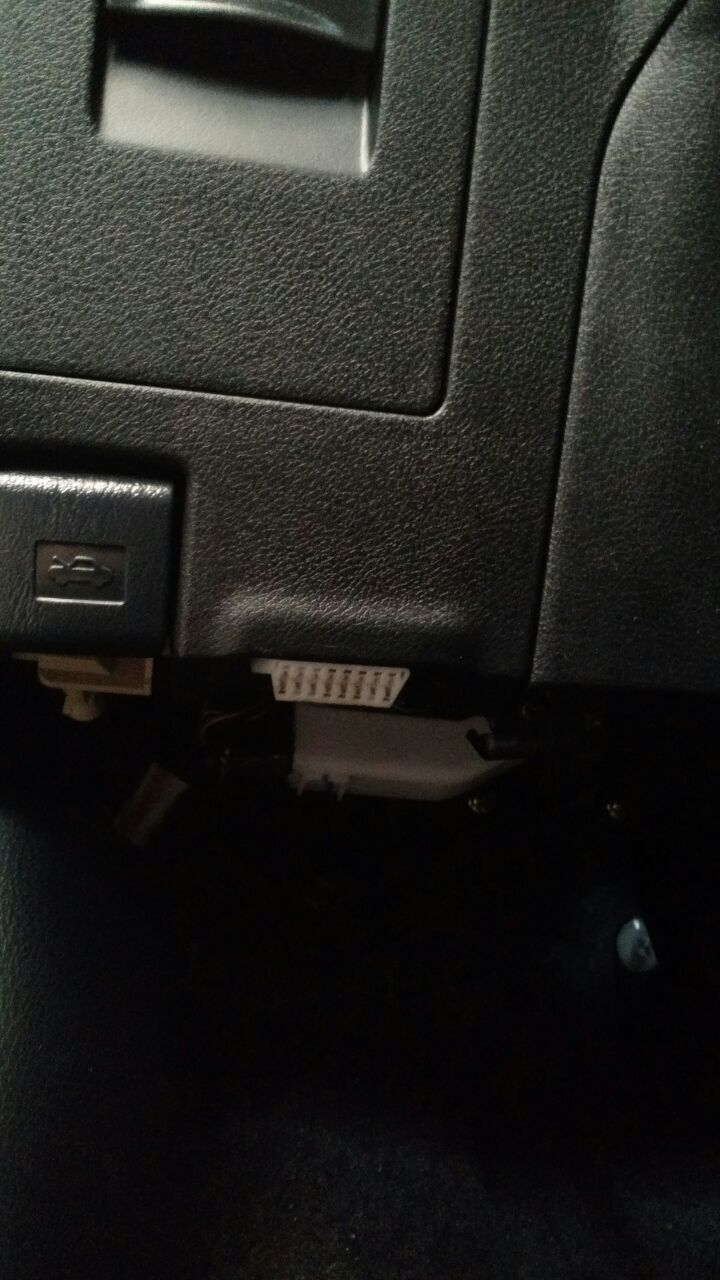
\includegraphics[scale=0.2]{obd} 
		\caption*{Fonte: Elaborada pelo autor, 2017.}
		\label{fig:obd}
\end{figure}

Uma discussão mais profunda sobre o uso destas placas e de outras é feita na seção \ref{sec:placasdedesenvolvimento}. 


Os últimos trabalhos a serem revisados são os que tiveram propostas mais relevantes e similares às propostas neste trabalho. Os trabalhos de conclusão de curso analisados (\cite{Dias2010}, \cite{Nunes2016} e \cite{Pereira2012}) tem propostas para criação de um sistema de telemetria para a modalidade Baja/fórmula SAE com um cenário similar ao deste trabalho. Primeiramente, \citeonline{Dias2010} tem como foco a pesquisa, projeto e execução da parte de \textit{hardware} do sistema de telemetria, deixando a parte de \textit{software} para um segundo trabalho. Já \citeonline{Nunes2016} utiliza parte do que já foi projetado em outros anos na equipe Car-Kará para projetar um sistema completo de telemetria com duas ECUs, incluindo \textit{software} e \textit{hardware}. Por último \citeonline{Pereira2012} traz uma abordagem diferenciada na qual é proposta uma revisão do projeto de elétrica da equipe de fórmula SAE da USP para introdução de conceitos de engenharia de \textit{software}.

Em \citeonline{Dias2010} é construído um sistema protótipo para toda a parte de eletrônica, instrumentação e telemetria do veículo UFVbaja. Os sensores que são instalados no veículo são de temperatura, combustível, bateria, velocidade e rotação do motor. O texto traz uma revisão de conceitos de eletrônica, principalmente da parte de microcontroladores, visto que essa é a área abordada pelo trabalho. É comentado sobre conversores analógico-digital, comunicação serial assíncrona, microcontroladores, USB e transceptores sem fio. Este último possui algumas informações sobre o protocolo ZigBee, este que é usado para enviar e receber dados entre os sistemas do veículo e dos boxes. É comentado que o protocolo oferece um excelente imunidade a interferências e a pode hospedar mais de 65 mil dispositivos, além de possuir taxas de transferências de dados entre 20Kbps e 250Kbps. Depois de explicar estes conceitos inicias, o trabalho explica quais e como funcionam os transdutores utilizados no mesmo. Para grandeza de velocidade e RPM foi escolhido um transdutor indutivo acoplado no eixo do motor para a rotação e na roda dianteira para a velocidade. Um fato curioso é que no veículo Baja da equipe Velociraptor, a medida da grandeza é feita na roda traseira, não na dianteira, isto é interessante pois aqui é comentado que a medida é tirada da roda dianteira devido ao fato do motor estar acoplado ao eixo traseiro e em casos de derrapagem o medidor de velocidade iria indicar um falso valor, porém também existe o problema de manutenção na roda dianteira, visto que acoplar sensores no eixo frontal é mais complicado por questões de apoio para os sensores. Para o nível de combustível é utilizado um transdutor de pressão diferencial, este fica acoplado na derivação da mangueira de combustível entre o tanque e o carburador do motor. O cálculo do nível de combustível é feito levando em conta a pressão que a gasolina exerce no fundo do tanque. Para medir a temperatura do motor é utilizado um sensor LM35 na carcaça externa do motor. Para se obter a tensão da bateria não existe um sensor específico, porém o trabalho utiliza o sinal proveniente da bateria, conectado diretamente em um canal ADC do microcontrolador. No \textit{firmware} do microcontrolador é realizado um cálculo com uma constante restauradora e assim é obtido o decaimento da tensão. Este cálculo de tensão da bateria não é gerado atualmente no Velociraptor e pode ser adicionado ao \textit{software} de tratamento de dados porém como um extra para testes, pois a bateria usada é calculada previamente para durar o tempo de prova. A configuração do SCOB possui um microcontrolador PIC16F877A e um PIC16F628A, ambos da Microship, a programação dos mesmos é feita em linguagem C. Para utilizar o protocolo ZigBee, é empregado o módulo Xbee-PRO. Este módulo tem potência de transmissão de 100mW e alcance de $1,6$ quilômetros sem contar com obstáculos segundo o autor. O sistema de boxes é independente e portátil, contando com um painel LCD de duas linhas e 16 colunas e LEDs para alertar sobre alguns dados específicos. Apesar de funcionar sem um computador, os dados recebidos pelo modulo Xbee-PRO podem ser enviados pelo microcontrolador para um computador via USB, e lá eles podem ser tratados para análise. Após estabelecida conexão com USB, são enviados pacotes com letras (que indicam a grandeza) e números (que indicam os valores medidos) e cada grandeza é separada por um caractere especial "\$". O trabalho é finalizado com uma discussão de resultados e algumas sugestões de aprimoramento como troca dos microcontroladores citados por outros com maior numero de periféricos além de maior poder de processamento e melhoria de precisão da medida do nível do combustível. Ambas as sugestões devem ser acatadas com a utilização dos microcontroladores mais recentes disponíveis no mercado e um método de medida de nível de combustível diferente do citado no trabalho (detalhes na seção \ref{subsec:combustivel}).

O trabalho de \citeonline{Nunes2016} cria um sistema para aquisição de dados de um veículo Baja, utilizando protocolo de comunicação CAN entre os múltiplos SCOBs presentes. O sistema tem uma proposta de utilização de arquitetura distribuída na qual são utilizados dois microcontroladores para aquisição de dados, diferentemente da maioria dos trabalhos revisados até agora. Um fica na parte dianteira e outro na traseira, também existe um terceiro microcontrolador, porém este só reune as informações mais importantes e disponibiliza em um painel digital. O trabalho cita algumas vantagens de se usar um sistema distribuído como diminuição no tamanho do chicote elétrico devido ao SCOB estar próximo aos sensores, facilidade de inserir novos módulos e maior robustez contra falhas elétricas. O último fator citado (robustez) é questionável pois a adição de novos sistemas aumentam a complexidade da manutenção do equipamento. Também são citados pontos negativos na utilização desta arquitetura, estes seriam o maior custo monetário para o projeto e maior complexidade de preparo do equipamento com uso do protocolo CAN. Os sensores utilizados no trabalho trabalham com grandezas como RPM, temperatura, nível do combustível, tensão da bateria e velocidade. As técnicas de medida das grandezas dos sensores de RPM, temperatura do motor, tensão da bateria e velocidade do veículo são as mesma das citadas no trabalho de \citeonline{Dias2010}, a única diferença encontrada está no nível de combustível, que é medido com um boia automotiva. Depois é comentado sobre o uso do protocolo CAN, tempo de bit e quadro de dados de uma mensagem do protocolo. O autor então comenta sobre a implementação e experimento, falando sobre os testes realizados sobre o sistema em bancada e em campo. O código dos SCOBs é feito em C e são utilizados dois Arduino Uno para a aquisição de dados dos sensores e um Arduino Mega para disponibilização dos dados no painel principal. O trabalho não possui um \textit{software} para tratamento dos dados recebidos e análise dos mesmos e também, contrário ao que o título indica, não existe um sistema de telemetria para os dados, apenas da aquisição dos mesmo. A ideia de utilização de múltiplos microprocessadores pode ser levada em consideração, principalmente devido ao tamanho de algumas plataformas como Arduino Nano e Raspberry Pi Zero, uma discussão sobre as plataformas de prototipagem e microcontroladores utilizados pode ser vista na seção \ref{sec:microcontroladores}.

O último trabalho é de \citeonline{Pereira2012}. Diferentemente dos outros, este não tem como objetivo criar um sistema de aquisição de dados de sensores de forma alguma, mas ele utiliza um sistema já concebido previamente e sugere conceitos de engenharia de \textit{software} que podem ser empregados neste meio do automobilismo. O objetivo em utilizar estes conceitos é adotar um padrão para ser seguido e facilitar a adequação do \textit{software} a evoluções. São apresentados alguns modelos de processo como modelo em cascata, desenvolvimento evolucionário e engenharia baseada em componentes, e por fim é demonstrado modelo feito especificamente para atender as necessidades desse projeto. O modelo criado possui uma execução de processos em círculo, aonde é inicialmente feita uma especificação dos \textit{software}, em cima dela é produzido um código, depois são realizados testes e por último é realizada uma manutenção, para logo após reiniciar o ciclo para implementar novas funcionalidade. As quatro fases citadas acima são especificadas no texto, a fase de especificações do \textit{software} tem os requisitos do mesmo levantados e avaliados, ela pode ser detalhada em quatro outras fase, de estudo de viabilidade, de elicitação e análise de requisitos, especificações dos requisitos e validação dos requisitos. A etapa de projeto de \textit{software} faz uma análise também dividida em quatro fases, primeiro é feito um projeto de arquitetura, depois projeto de componentes, projeto de estrutura de dados e por último o projeto do algoritmo. A etapa de testes é na qual o sistema é avaliado, verificando se ele esta de acordo com os requisitos estudados. Por último a etapa de manutenção consiste em adequar e manter o ambiente criado nas últimas etapas, reparando defeitos de \textit{software}, adaptando-o para novos ambientes operacionais e adicionando funcionalidades. O trabalho especifica alguns pontos dentro das etapas comentadas acima, porém elas são relativas ao modelo adotado pelo autor e não são de uso geral. Finalizando, o autor conclui que para trabalhos futuros é possível atingir padrões como ISO9126 de qualidade, além de controle de custos através da verificação de diversas propostas de arquitetura. 

\section{Conclusão de capítulo}
A partir do que foi discutido neste capítulo, foram retiradas algumas conclusões sobre os trabalhos citados. Os trabalhos mais relacionados possui algumas características específicas que podem ser citadas em relação ao trabalho de proposto, como alguns pontos onde estes trabalhos se equivalem e outros pontos no qual os trabalhos divergem. 

Inicialmente, sobre os pontos que se equivalem, todos os trabalhos implementam sistemas de aquisição de dados. Este sistema é ponto chave para recolher os dados medidos a partir dos sensores distribuídos pelo veículo. Outro ponto importante é que estes trabalhos implementam os seus sistemas de aquisição e sensores de forma customizada. Isto quer dizer que esta característica permite com que os componentes e sensores sejam alterados conforme o escopo trabalhado pelos autores, adicionando novas funcionalidades ou mantendo as que já existem, sem necessidade de terceiros. Também pode ser destacado o fato de algum destes trabalhos possuírem arquitetura distribuída de microcontroladores. A utilização de \textit{N} microcontroladores no veículo permite uma melhor manutenção do mesmo devido a melhor distribuição dos sensores e da fiação elétrica, além de melhor desempenho pois um microcontrolador fica encarregado de tratar os dados de uma parcela menor de sensores.

Em relação as características que estes trabalhos não possuem, é destacável a falta de especificação do \textit{software}. Por ter o foco na parte de aquisição, pouco se fala sobre as funcionalidades do sistema de tratamento de dados. Isto implica em outras duas características, a falta de clareza sobre a exposição das informações com gráficos para melhor entendimento dos mesmos pelos usuários e também a modularidade da disposição das informações, mostrando apenas dados interessantes para o momento.  
